\documentclass{article}
\usepackage[utf8]{inputenc}
\usepackage[english]{babel}
\usepackage{amsmath}
\usepackage[]{amsthm}
\usepackage[]{amssymb} 
\usepackage{mathrsfs}
\usepackage{tcolorbox}
\usepackage{nicefrac}
\usepackage{mathtools}
% \usepackage{graphicx}
\usepackage{caption}
\usepackage{subcaption}
\usepackage{array}

\graphicspath{ {./images/} }

\theoremstyle{definition}
\newtheorem*{claim}{Claim}
\newtheorem*{corollary}{Corollary}
\DeclareMathOperator{\adj}{\operatorname{adj}}
\DeclareMathOperator{\im}{\operatorname{im}}
\DeclareMathOperator{\spn}{\operatorname{span}}
\DeclareMathOperator{\nll}{\operatorname{null}}
\newcommand{\trace}{\operatorname{trace}}
\newcommand{\R}{\mathbb{R}}
\newcommand{\Z}{\mathbb{Z}}
\newcommand{\N}{\mathbb{N}}
\newcommand{\F}{\mathbb{F}}
\newcommand{\C}{\mathbb{C}}
\newcommand{\D}{\operatorname{D}}
\newcommand{\GL}{\operatorname{GL}}
\newcommand{\SL}{\operatorname{SL}}
\newcommand{\GLnR}{\GL_n(\R)}
\newcommand{\SLnR}{\SL_n(\R)}
\DeclarePairedDelimiter\floor{\lfloor}{\rfloor}
\DeclarePairedDelimiter\set{\{}{\}}
\DeclarePairedDelimiter\abs{\lvert}{\rvert}
\DeclarePairedDelimiter\genby{\langle}{\rangle}
\DeclarePairedDelimiter\bilform{\langle}{\rangle}
\newcommand{\restrict}[1]{ \big|_{#1} }
\newcommand{\evalat}[2]{\Big|_{#1}^{#2}}


\title{18.701: Problem Set 10}
\author{Dmitry Kaysin}
\date{August 2020}
\begin{document}
\maketitle 


\subsection*{Problem 1}

\begin{tcolorbox}
a) Let $\SL_2$ be the special linear group of real matrices with determinant $1$.
Determine the possible eigenvalues $\lambda$ (real or complex) of the elements of $\SL_2$, and make a drawing showing the points $\lambda$ in the complex plane.
\end{tcolorbox}

We start with $2 \times 2$ matrix of the form
\[
    A =
    \begin{pmatrix}
        a & b \\
        c & d
    \end{pmatrix}
\]
with $\det A = ad - bc = 1$.

Characteristic polynomial of $A$ is $t^2 - tr + 1$ where $r = \trace A = a+d$.
Eigenvalues of $A$ are thus
\[
    \lambda = \frac{r \pm \sqrt{r^2-4}}{2}.
\]
As $r \to \infty : \lambda \to \pm \infty$ and
as $r \to -\infty : \lambda \to \pm 0$.
For $r$ in the interval $(\-\infty, -2] \cup [2, \infty)$ eigenvalues of $A$ are real.
For $r$ in the interval $(-2, 2)$ eigenvalues of $A$ are complex, occur in conjugate pairs and their locus is upper and lower half of the unit circle of the complex plane.

\begin{figure}[h]
    \caption{Possible eigenvalues of $A \in \SL_2$ in the complex plane.}
    \centering
    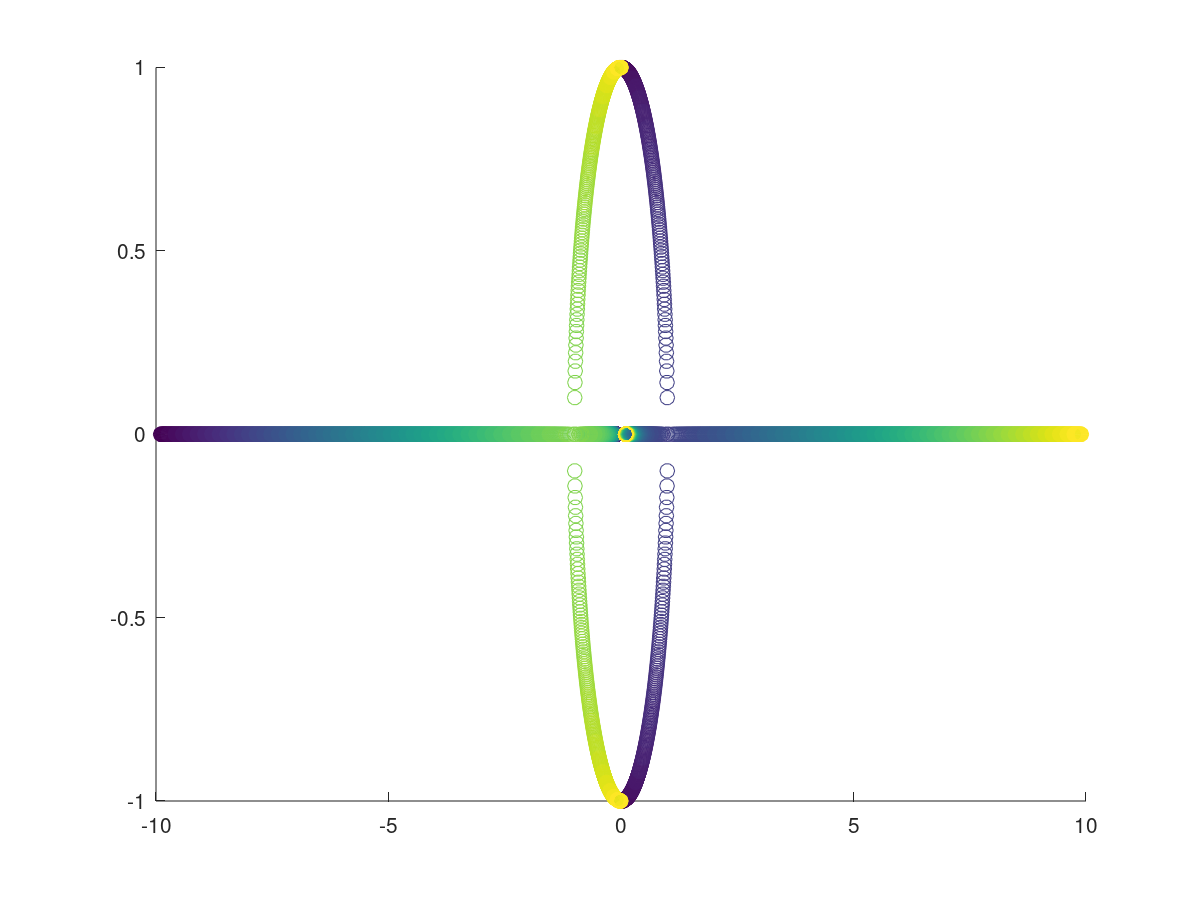
\includegraphics[width=0.8\textwidth]{ps10p1}
\end{figure}


\begin{tcolorbox}
b) For each $\lambda$, decompose the set of matrices $P \in \SL_2$ with eigenvalue $\lambda$ into $\SL_2$-conjugacy classes.
\end{tcolorbox}

\begin{proof}
Conjugate matrices have the same characteristic polynomial and the same eigenvalues.
\end{proof}

\begin{tcolorbox}
c) Determine the matrices $P \in \SL_2$ that can be obtained as $P = e^A$ for some real matrix $A$.
\end{tcolorbox}

\begin{proof}
\end{proof}

\subsection*{Problem 2}

\begin{tcolorbox}
\end{tcolorbox}

\begin{proof}
\end{proof}


\end{document}
